\chapter{Lab Page tables:页表实验}
\begin{introduction}
    \item 使用页表机制加速系统调用
    \item 打印页表
    \item 追踪被访问的页
    \item RISC-V 的页表机制
\end{introduction}

在上一个实验中,我们初次修改 xv6 的内核,为其添加了两个系统调用。本次实验的重点则是在于操作系统的另一个机制:页表。在本次实验中,我们会初探页表的一些性质,并利用页表机制完成一些任务。

\section{使用页表机制加速系统调用}

在现实的操作系统中,很多系统调用只是读取内核态的一些数据结构,而并不进行写入操作,这类系统调用的一个典型例子就是 getpid 系统调用。对于这类系统调用,诸如 Linux 等操作系统不会将内核的数据结构复制到用户空间,而是直接将存放该数据结构的页通过页表的机制映射到用户空间的对应位置,从而免去了复制的开销,提高了系统的性能。

本实验中,需要在进程创建时将一个内存页面以只读权限映射到 \lstinline{USYSCALL} 位置(参见 \lstinline{memlayout.h})中的定义。该映射的页面开头存储有内核数据结构 \lstinline{struct usyscall} ,该数据结构在进程创建时被初始化,并且存储有该进程的 pid 。在这个实验中,我们使用纯用户空间的函数 \lstinline{ugetpid()} 来替代需要进行内核态到用户态拷贝的 getpid 系统调用。户空间的函数 \lstinline{ugetpid()} 已经在用户空间中被实现了,我们需要做的是将映射页面的工作完成。

由于需要在创建进程时完成页面的映射,故而我们考虑修改 \lstinline{kernel/proc.c} 中的 \lstinline{proc_pagetable(struct proc *p)} ,即用于为新创建的进程分配页面的函数。在 \lstinline{proc_pagetable()} 完成分配新的页面后,即可以使用 \lstinline{mappages} 函数分配页面:
\begin{lstlisting}[language=C]
pagetable_t
proc_pagetable(struct proc *p)
{
  pagetable_t pagetable;

  // An empty page table.
  pagetable = uvmcreate();
  if(pagetable == 0)
    return 0;

  //map a user read only page at USYSCALL, for optimization for the getpid()
  if(mappages(pagetable, USYSCALL, PGSIZE,
              (uint64)(p->usyscall), PTE_R | PTE_U) < 0){
    uvmfree(pagetable, 0);
    return 0;
  }
......
\end{lstlisting}

页面映射时,需要设定其权限为只读,故权限位为 \lstinline{PTE_R | PTE_U} ,此后在 \lstinline{allocproc()} 中添加初始化该页面,向其中写入数据结构的代码:
\begin{lstlisting}[language=C]
......
  // Allocate a usyscall page.
  if((p->usyscall = (struct usyscall *)kalloc()) == 0){
    freeproc(p);
    release(&p->lock);
    return 0;
  }
  p->usyscall->pid = p->pid;
......
\end{lstlisting}
\begin{theorem}[注意加锁] 
    当在内核态下操作进程相关的数据结构时,由于可能出现并发读写的情况,故而我们需要先获取该数据结构的锁,然后再进行操作,最后释放该锁;否则可能造成竞争读写,导致数据不一致的情况出现。
\end{theorem}

在完成页面的初始化后,进程应当得以正常运行,但需要记得在进程结束后释放分配的页面,该动作在 \lstinline{freeproc()} 中进行,添加的代码如下:
\begin{lstlisting}[language=C]
......
  if(p->usyscall)
    kfree((void*)p->usyscall);
  p->usyscall = 0;
......
\end{lstlisting}

当考虑好进程的页面分配,页面初始化和页面回收后,映射页面的工作就全部完成了。编译并启动 xv6 后,在 shell 中运行 \lstinline{pgtbltest} ,即可看到预期的输出:
\begin{lstlisting}
$ pgtbltest
ugetpid_test starting
ugetpid_test: OK
......
\end{lstlisting}

\section{打印页表}

为了方便将页表的内容可视化,我们需要实现一个名为 \lstinline{vmprint()} 的函数,其接受一个 \lstinline{pagetable_t} 类型的参数,并按下面的格式打印页表:
\begin{lstlisting}
page table 0x0000000087f6e000
 ..0: pte 0x0000000021fda801 pa 0x0000000087f6a000
 .. ..0: pte 0x0000000021fda401 pa 0x0000000087f69000
 .. .. ..0: pte 0x0000000021fdac1f pa 0x0000000087f6b000
 .. .. ..1: pte 0x0000000021fda00f pa 0x0000000087f68000
 .. .. ..2: pte 0x0000000021fd9c1f pa 0x0000000087f67000
 ..255: pte 0x0000000021fdb401 pa 0x0000000087f6d000
 .. ..511: pte 0x0000000021fdb001 pa 0x0000000087f6c000
 .. .. ..509: pte 0x0000000021fdd813 pa 0x0000000087f76000
 .. .. ..510: pte 0x0000000021fddc07 pa 0x0000000087f77000
 .. .. ..511: pte 0x0000000020001c0b pa 0x0000000080007000
\end{lstlisting}

实现了 \lstinline{vmprint()} 之后,我们可以在 \lstinline{kernel/exec.c} 中的 \lstinline{exec()} 函数的 \lstinline{return argc} 前加入 \lstinline{if(p->pid==1) vmprint(p->pagetable)} ,即可打印 pid 为 1 的进程的页表。

为了方便使用其它与页表相关的函数,我们在 \lstinline{kernel/vm.c} 中实现 \lstinline{vmprint()} 函数。在实现该函数前,我们根据 xv6 实验手册的提示,首先阅读 \lstinline{freewalk} 函数的实现以供参考:
\begin{lstlisting}[language=C]
// Recursively free page-table pages.
// All leaf mappings must already have been removed.
void
freewalk(pagetable_t pagetable)
{
  // there are 2^9 = 512 PTEs in a page table.
  for(int i = 0; i < 512; i++){
    pte_t pte = pagetable[i];
    if((pte & PTE_V) && (pte & (PTE_R|PTE_W|PTE_X)) == 0){
      // this PTE points to a lower-level page table.
      uint64 child = PTE2PA(pte);
      freewalk((pagetable_t)child);
      pagetable[i] = 0;
    } else if(pte & PTE_V){
      panic("freewalk: leaf");
    }
  }
  kfree((void*)pagetable);
}
\end{lstlisting}

不难发现,该函数通过递归的方式逐层释放页表。仿照这种递归方式,对该函数略做修改,我们可以构造遍历页表并按层数格式打印的函数 \lstinline{vmprintwalk(pagetable_t pagetable, int depth)} :
\begin{lstlisting}[language=C]
void
vmprintwalk(pagetable_t pagetable, int depth)
{
  // there are 2^9 = 512 PTEs in a page table.
  for(int i = 0; i < 512; i++){
    pte_t pte = pagetable[i];
    if((pte & PTE_V) && (pte & (PTE_R|PTE_W|PTE_X)) == 0){
      // this PTE points to a lower-level page table.
      for (int n = 0; n < depth; n++)
        printf(" ..");
      printf("%d: pte %p pa %p\n", i, pte, PTE2PA(pte));
      uint64 child = PTE2PA(pte);
      vmprintwalk((pagetable_t)child, depth+1);
    } else if(pte & PTE_V){
      for (int n = 0; n < depth; n++)
        printf(" ..");
      printf("%d: pte %p pa %p\n", i, pte, PTE2PA(pte));
    }
  }
}
\end{lstlisting}

然后实现 \lstinline{vmprint()} 函数时,只需给定初始深度为 1 ,调用 \lstinline{vmprintwalk(pagetable_t, int)} 即可:
\begin{lstlisting}[language=C]
void
vmprint(pagetable_t pagetable)
{
  printf("page table %p\n",pagetable);
  vmprintwalk(pagetable,1);
}
\end{lstlisting}

最后按照要求在 \lstinline{kernel/exec.c} 中的 \lstinline{exec()} 函数的 \lstinline{return argc} 前加入 \lstinline{if(p->pid==1) vmprint(p->pagetable)} :
\begin{lstlisting}[language=C]
......
    if(p->pid==1) vmprint(p->pagetable);
    return argc; // this ends up in a0, the first argument to main(argc, argv)
......
\end{lstlisting}

编译并启动 xv6 后 ,即可看到预期的输出,如下图所示:
\begin{figure}[H]
  \centering
  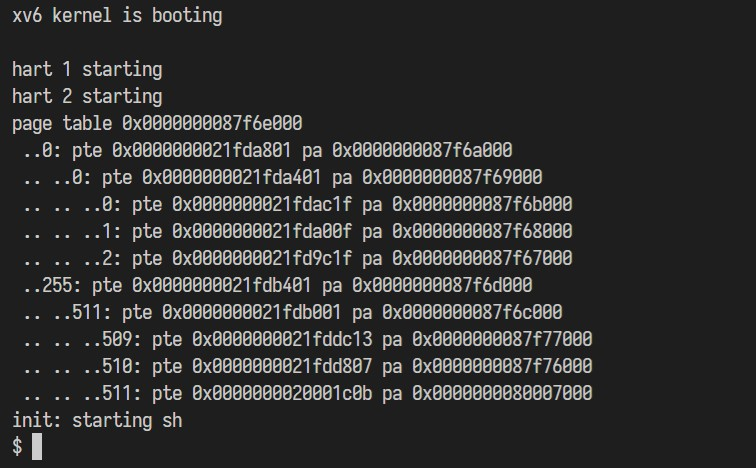
\includegraphics[width=0.8\textwidth]{pgtbl_vmprint.jpg}
  \caption{ \lstinline{vmprint()} 的输出结果}
\end{figure}

\section{追踪被访问的页}

现代很多编程语言都具备了内存垃圾回收的功能( GC , garbage collect ),而垃圾回收器功能的实现则需要得到一个页面自上次检查后是否被访问的信息。实现这种功能可以是纯软件的,但其效率低下;而利用页表的硬件机制(访问位)和操作系统相结合,在 xv6 中添加一个系统调用 \lstinline{pgaccess()} 用以读取页表的访问位并传递给用户态程序,从而告知他们一些内存页面自上次检查以来的访问情况,是一个较好的方法。

我们需要实现的 \lstinline{pgaccess()} 系统调用接受 3 个参数:第一个参数为需要检查页面的初始地址,第二个参数是从初始地址向后检查多少个页面,第三个参数则是一个指针,指向用于存储结果的位向量的首地址。

首先,按照前文提及的方法添加系统调用以及其在 \lstinline{kernel/sysproc.c} 中的实现 \lstinline{sys_pgaccess()} ,并使用 \lstinline{argint()} 和 \lstinline{argaddr()} 获取传入的参数:
\begin{lstlisting}[language=C]
int sys_pgaccess(void)
{
  uint64 srcva, st;
  int len;
  uint64 buf = 0;
  struct proc *p = myproc();

  acquire(&p->lock);

  argaddr(0, &srcva);
  argint(1, &len);
  argaddr(2, &st);
  ......
  return 0;
}
\end{lstlisting}

之后,对获取的参数进行预处理后,对每个需要检查的页面,使用 \lstinline{kernel/vm.c} 中提供的 \lstinline{walk(pagetable_t, uint64, int)} 来获取其页表项,重置该页表的 \lstinline{PTE_A} 访问位,并使用位运算将其访问状态置入临时位向量中;最后将临时位向量拷贝至用户内存空间指定的地址中。笔者的完整的实现如下:
\begin{lstlisting}[language=C]
extern pte_t *walk(pagetable_t, uint64, int);
int sys_pgaccess(void)
{
  // lab pgtbl: your code here.
  uint64 srcva, st;
  int len;
  uint64 buf = 0;
  struct proc *p = myproc();

  acquire(&p->lock);

  argaddr(0, &srcva);
  argint(1, &len);
  argaddr(2, &st);
  if ((len > 64) || (len < 1))
    return -1;
  pte_t *pte;
  for (int i = 0; i < len; i++)
  {
    pte = walk(p->pagetable, srcva + i * PGSIZE, 0);
    if(pte == 0){
      return -1;
    }
    if((*pte & PTE_V) == 0){
      return -1;
    }
    if((*pte & PTE_U) == 0){
      return -1;
    }
    if(*pte & PTE_A){
      *pte = *pte & ~PTE_A;
      buf |= (1 << i);  
    }
  }
  release(&p->lock);
  copyout(p->pagetable, st, (char *)&buf, ((len -1) / 8) + 1);
  return 0;
}
\end{lstlisting}

\begin{theorem}[再次提醒加锁] 
    页表也是内核数据结构,可能被多个处理器同时操作,故记得加锁。
\end{theorem}

至此, \lstinline{pgaccess()} 系统调用实现完成。编译并启动 xv6 后,在 shell 中运行 \lstinline{pgtbltest} ,即可看到预期的输出,如下图所示:
\begin{figure}[H]
  \centering
  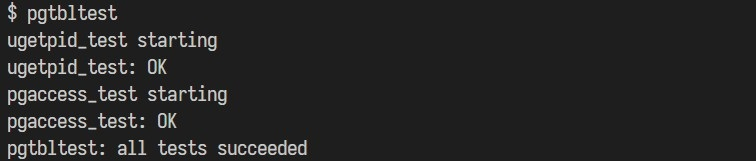
\includegraphics[width=0.8\textwidth]{pgtbl_pgaccess.jpg}
  \caption{ pgaccess 的测评结果}
\end{figure}

\paragraph*{实验结果} 在完成 Lab Page tables 中的所有实验后,根据 MIT 6.S081 的传统,需要在实验目录下创建一个名为 \lstinline{time.txt} 文本文件,其中只包含一行,为完成该实验的小时数。然后在终端中执行 \lstinline{make grade} ,即可对整个实验进行自动评分,笔者的结果如下:
\begin{figure}[H]
  \centering
  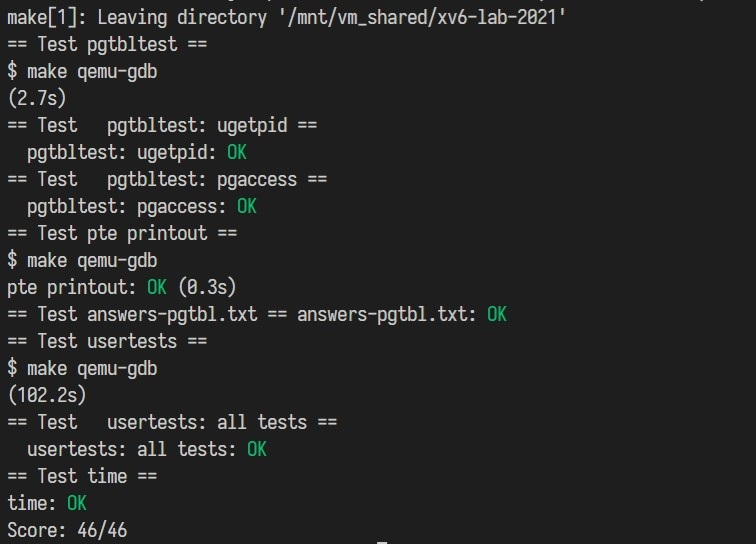
\includegraphics[width=0.8\textwidth]{pgtbl_grade.jpg}
  \caption{ Lab Page tables 的测评结果}
\end{figure}
可见测试全部通过,得分为满分。


\section{小结:RISC-V 的页表机制}

通过上面的几个实验,我们能够大致了解 RISC-V 的 MMU 硬件提供的分页机制与操作系统配合的全过程。但是,上面的实验里没有详细地总结 RISC-V 硬件的的分页机制,这里我们将参考 RISC-V 的手册 \textit{The RISC-V Instruction Set Manual: Volume II: Privileged Architecture} \footnote{\url{https://riscv.org/wp-content/uploads/2017/05/riscv-privileged-v1.10.pdf}} 对 RISC-V 中最常用的 Sv-39 ( Page-Based 39-bit Virtual-Memory System ) 分页机制进行一个小结。

\begin{figure}[H]
  \centering
  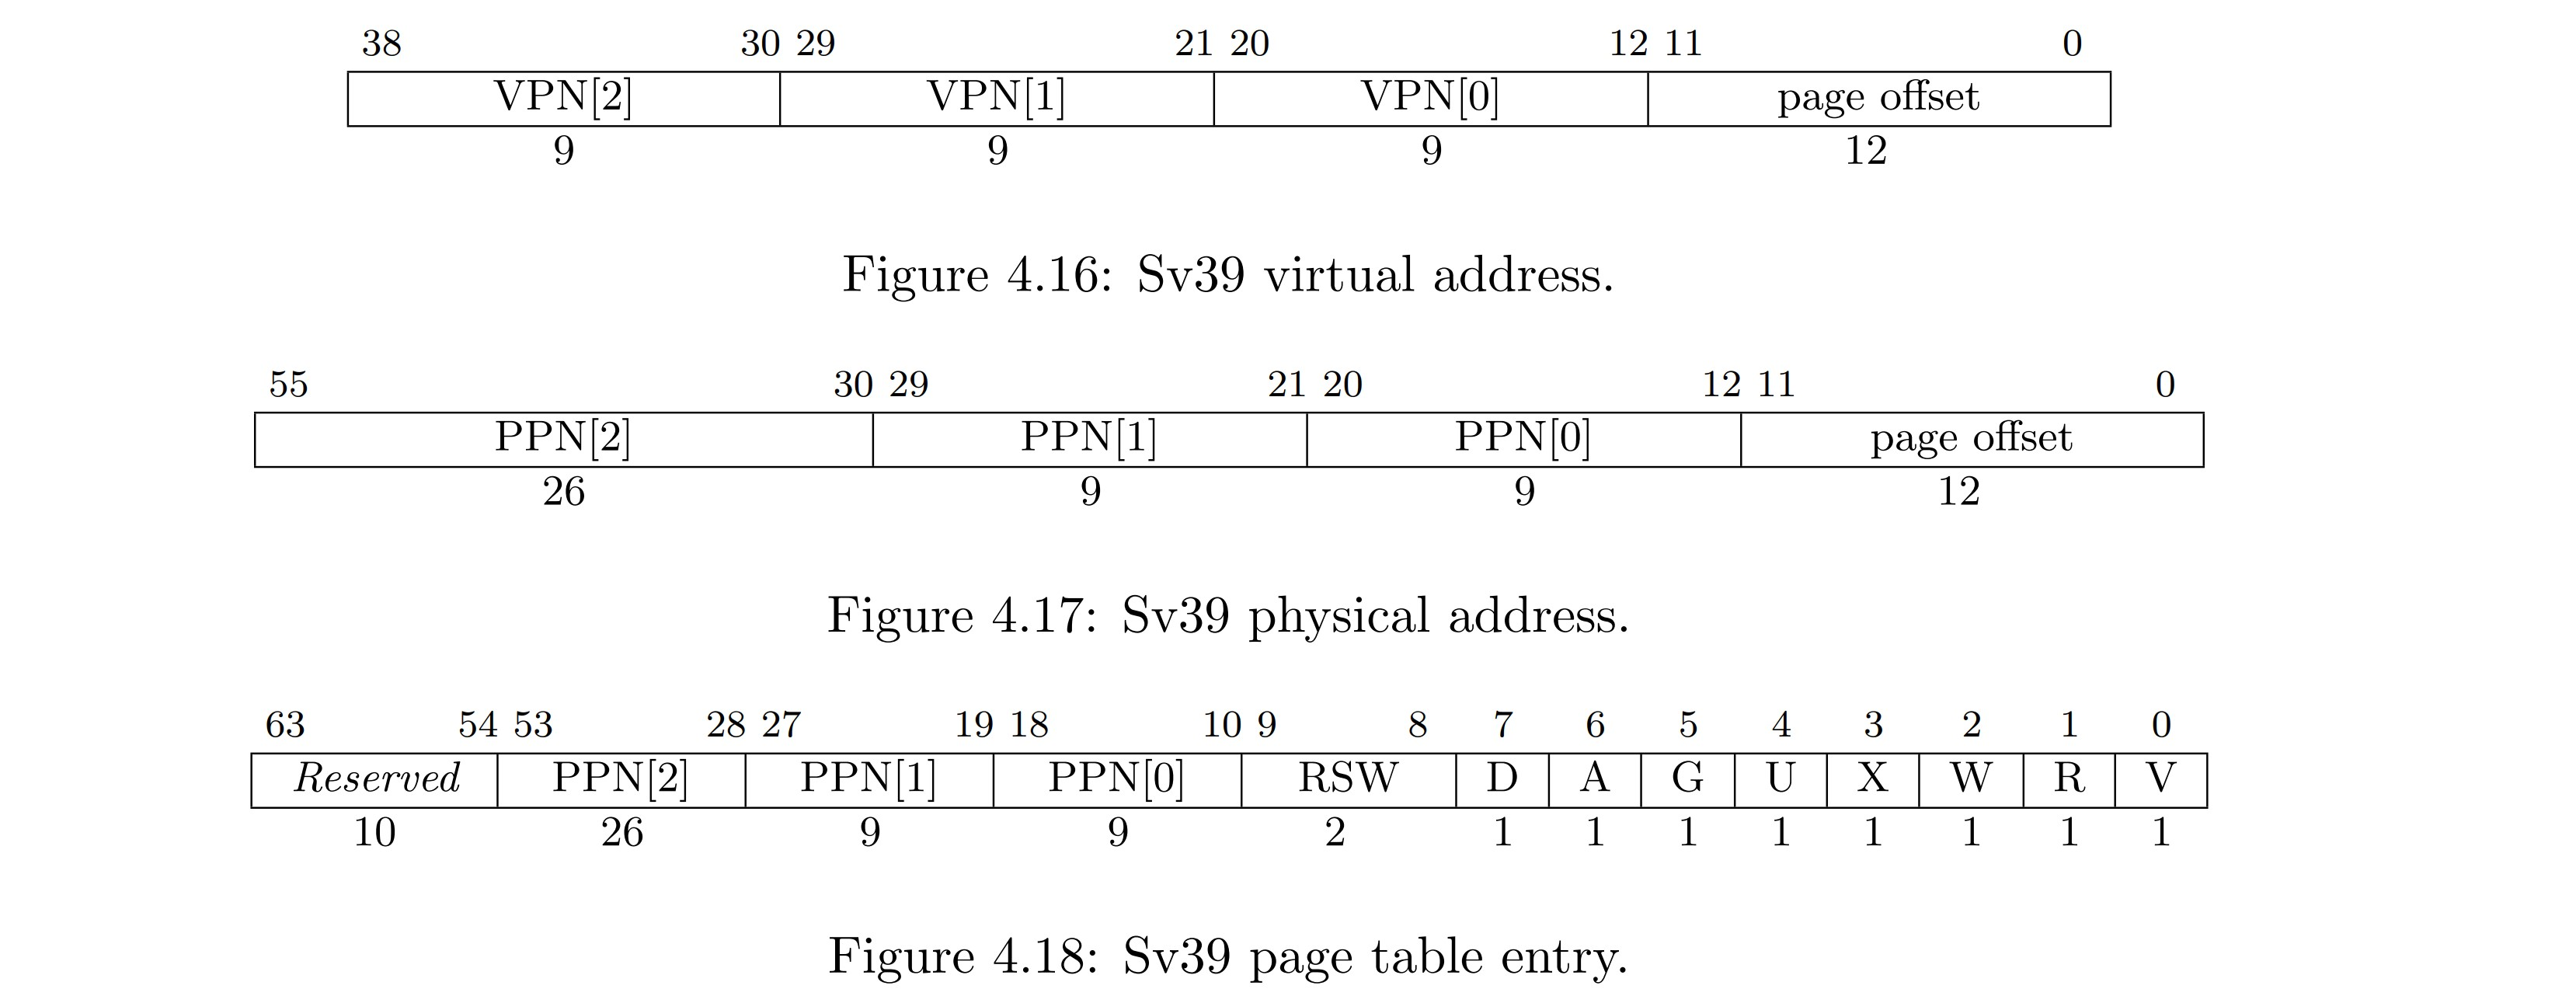
\includegraphics[width=1.0\textwidth]{pgtbl_sv39.jpg}
  \caption{ RISC-V 手册中关于 Sv-39 的图解(手册 p.63 ) }
\end{figure}

上图即RISC-V 手册中关于 Sv-39 的总结。参考对应上图中的 Figure 4.16 ,顾名思义, Sv-39 的支持 39 位的虚拟地址,即 64 位的低 39 位是有效的,高位均为第 38 位的值;其一个页面大小为 4KB (必须边界对齐,即页面起始地址的低 12 位必须均为 0 ) ,故整个 39 位的地址的 0 到 11 位是页内偏移,在地址变换时不发生变化。

除去页内偏移外,剩余高的 27 位被等分为了 3 段,每段各 9 位;每一段对应各级页表,故 Sv-39 是一个三级页表的系统 (比 x86 架构的 32 位二级页表要多一级),而每段的 9 位的 VPN (虚存页面编号)对应该级页表中的项,即每一个页表中有 $2^9 = 512$ 项,这与页面大小是匹配的,因为每个页表项为 64 位 (见上图中的 Figure 4.18 ),即 8 Byte ,故整个页表的大小恰好为 4KB ,即一页的大小。

在 Sv-39 中,物理地址的格式对应上图中的 Figure 4.17 ,与虚拟地址类似,页面大小为 4KB 且边界对齐;除了低位的 12 位页内偏移外,高位为物理的页号(共 44 位物理页号)。对于页表项,高位的未使用的 54 到 63 位始终置 0 ,而后是 44 位物理页号,而后的第 9 位和第 8 位是供操作系统自定义使用的,而后的第 0 到第 7 位是该页面的状态位、权限设置和属性等。具体的 0 到 7 位的含义如下:
\begin{itemize}
    \item 第 7 位, Dirty bit ,对应的页面被写入后会被硬件置为 1 ,可被操作系统置为 0
    \item 第 6 位, Access bit ,对应的页面被访问后会被硬件置为 1 ,可被操作系统置为 0
    \item 第 5 位, Global bit ,其为 1 表示该页表项的映射对所有的内存空间均有效
    \item 第 4 位到第 1 位, User/Read/Write/eXecute bit,用于控制页面的权限,由操作系统设置
    \item 第 0 位,Valid bit,页表项的有效位
\end{itemize}

在使用 Sv-39 分页机制进行内存地址转换时,根页表的物理页面号 PPN 会被存储在 SATP 寄存器的 PPN 号的区间内,且 SATP 寄存器的 MODE 段(分页模式)和 ASID 段(地址空间)都被设为进程对应的值。某个指令访问某个虚拟地址时,处理器会:
\begin{enumerate}
    \item 读取 SATP 寄存器的 PPN 对应的页表根页面,
    \item 然后依次沿着各级 VPN (虚存页面编号)找到虚拟地址对应的页表项,
    \item 检查权限无误后,根据指令的操作设置该页表项的 Dirty/Access 位,
    \item 并且用该页表项的 PPN 与指令的页内偏移拼接,得到物理地址,
    \item 然后执行指令的操作。
\end{enumerate}

更加形象化的表述如下图所示:
\begin{figure}[H]
  \centering
  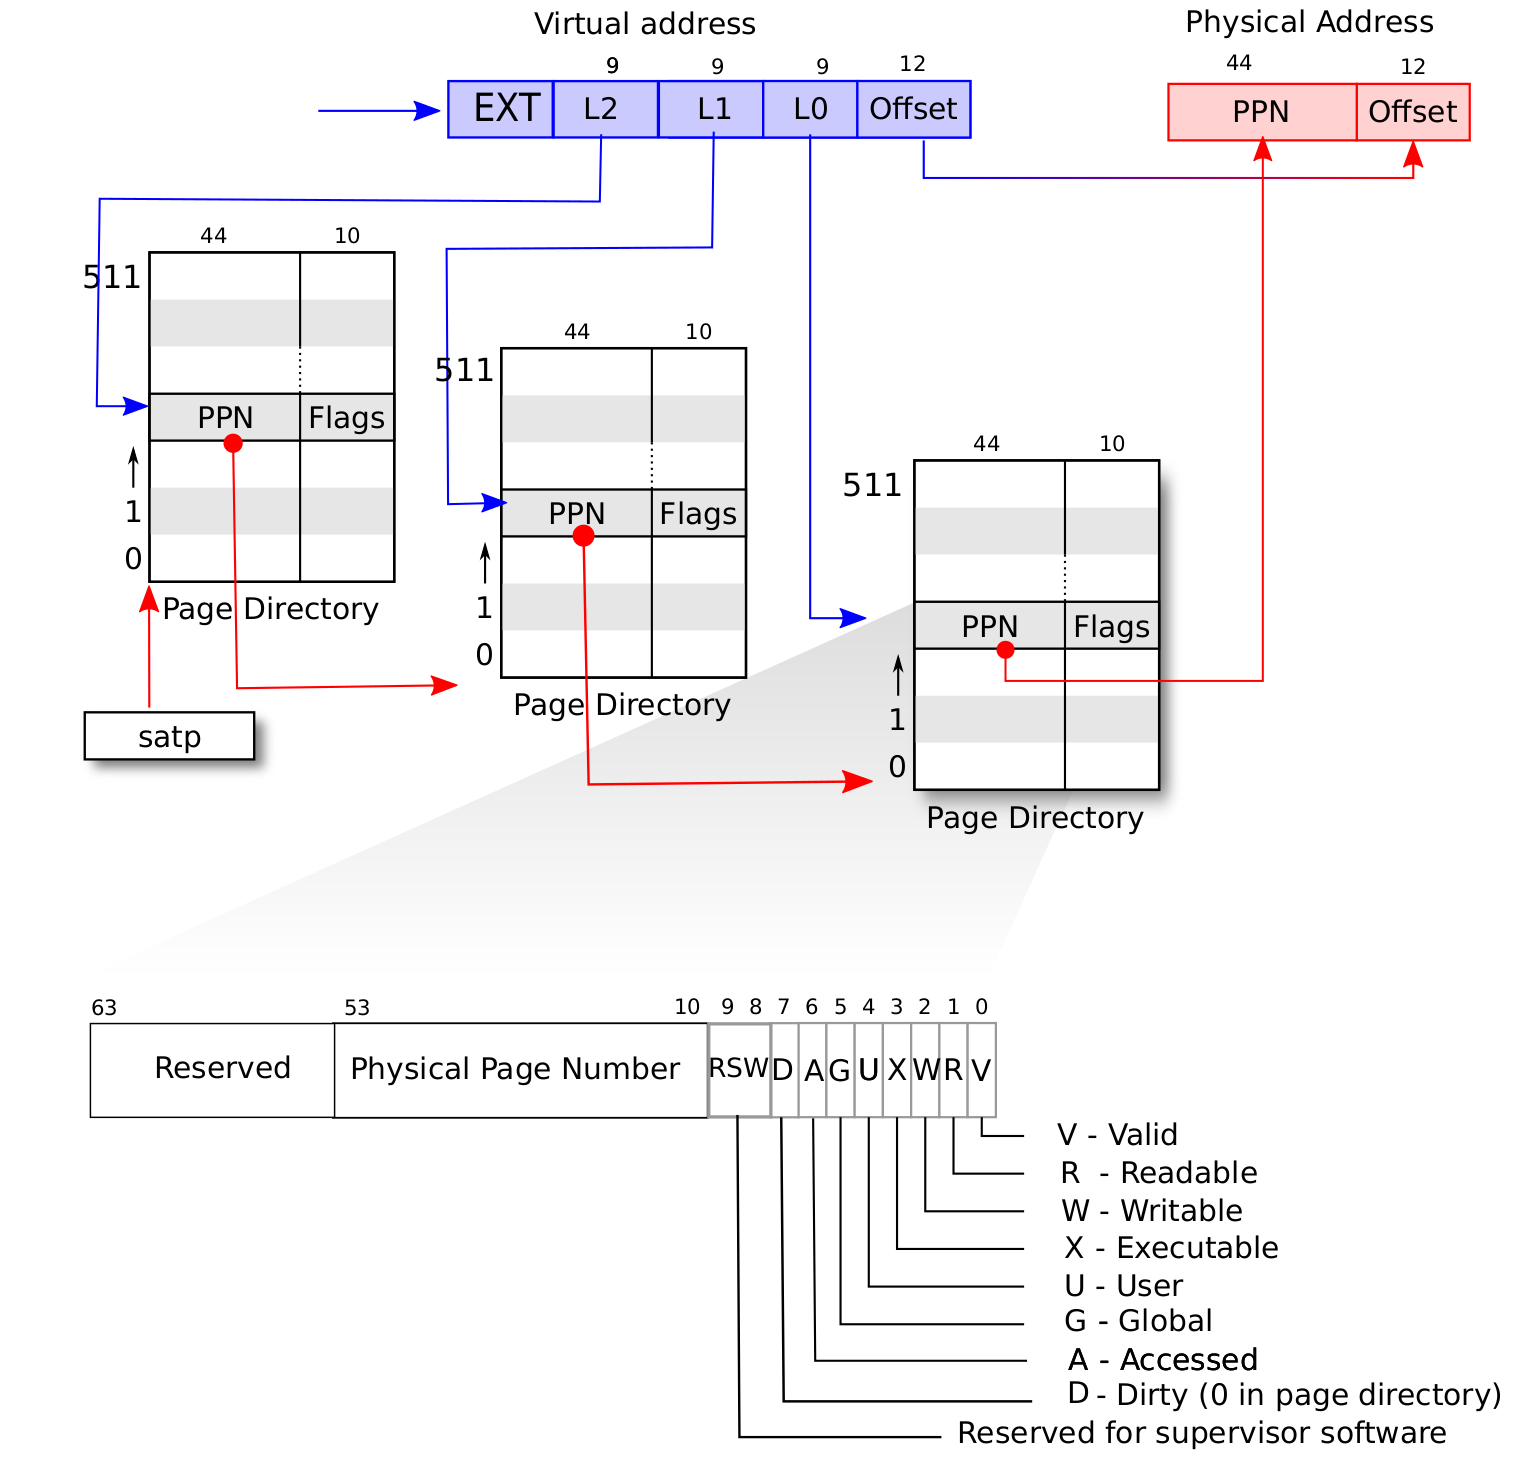
\includegraphics[width=0.8\textwidth]{pgtbl_sv39-full.png}
  \caption{ Sv-39 地址转换的过程(来源于 MIT 6.828 课程) }
\end{figure}

我们的 xv6 操作系统在 RISC-V 平台上借助的硬件分页机制就是 Sv39 ,若要将 xv6 移植到其它硬件平台上(如 s390x, 龙芯等),则需要根据其硬件提供的分页机制重写有关分页机制初始化和页表操作的代码。

\begin{proposition}[关于大页 ( Huge Page )]
    由于现代的应用软件占据的内存逐渐增大,主流的计算机硬件(如 x64 平台)逐渐开始支持较大的页面(如 x64 支持的 2MiB 的大页)。RISC-V 作为先进的架构,同样也在 Sv39 分页模式中支持大页,而且其支持两种不同尺寸的大页:大小为 2MiB 的页被称为 \textit{megapages} ,而大小为 1GiB 的页被称为 \textit{gigapages} 。这两类大页都需要进行边界对齐(例如一个 \textit{gigapage} 开始的物理地址和虚拟地址的低 30 位必须均为 0)。大页的机制提供了更好的访存性能,且可以很好地融入目前的 Sv39 分页模式中。
\end{proposition}

得益于硬件制造技术的进步, Sv-39 提供的 39 位虚拟地址空间和 56 位物理地址空间逐渐无法适应一些新的硬件:越来越多的计算机已经配置了超过 512 GiB 的物理内存(比如笔者的工作站,安装的物理内存为 1.5 TiB )。 RISC-V 除了提供 Sv-39 的分页机制外,同样也提供了基于四级页表的 Sv-48 分页机制。该机制支持 48 位的虚拟地址,且提供了 4KB , 2MB , 1GB和 512GB 四种可选的页面大小,预计足够未来数年的硬件使用。